% Created 2014-08-28 Thu 17:51
\documentclass[presentation]{beamer}
\usepackage[utf8]{inputenc}
\usepackage[T1]{fontenc}
\usepackage{fixltx2e}
\usepackage{graphicx}
\usepackage{longtable}
\usepackage{float}
\usepackage{wrapfig}
\usepackage{rotating}
\usepackage[normalem]{ulem}
\usepackage{amsmath}
\usepackage{textcomp}
\usepackage{marvosym}
\usepackage{wasysym}
\usepackage{amssymb}
\usepackage{hyperref}
\tolerance=1000
\hypersetup{pdfauthor="Vasilij Schneidermann", pdftitle="Emacs Lisp or Why Emacs' Extension Language Is Worth Another Look", colorlinks, linkcolor=black, urlcolor=blue}
\usetheme{Rochester}
\usecolortheme[RGB={87,83,170}]{structure}
\author{Vasilij Schneidermann}
\date{August 24, 2014}
\title{Emacs Lisp or Why Emacs' Extension Language Is Worth Another Look}
\hypersetup{
  pdfkeywords={},
  pdfsubject={},
  pdfcreator={Emacs 24.3.1 (Org mode 8.2.7c)}}
\begin{document}

\maketitle
\begin{frame}{Outline}
\tableofcontents
\end{frame}

\AtBeginSection{\frame{\sectionpage}}

\section{Introduction}
\label{sec-1}

\begin{frame}[label=sec-1-1]{Speaker}
\begin{itemize}
\item Vasilij Schneidermann, 22
\item Information systems student
\item Working at bevuta IT, Cologne
\item \texttt{v.schneidermann@gmail.com}
\item \url{https://github.com/wasamasa}
\end{itemize}
\end{frame}

\begin{frame}[label=sec-1-2]{Preliminary notes}
\begin{itemize}
\item Pretty subjective at times
\item Prepare for dogfooding
\end{itemize}
\end{frame}

\begin{frame}[label=sec-1-3]{What this talk will be about}
\begin{itemize}
\item Emacs features
\item Demonstrations of what Emacs can do
\item The community
\end{itemize}
\end{frame}

\begin{frame}[label=sec-1-4]{What this talk will not be about}
\begin{itemize}
\item Teaching you how to use Emacs
\item Editor wars
\end{itemize}
\end{frame}

\section{How I got started with Emacs and Emacs Lisp}
\label{sec-2}

\begin{frame}[label=sec-2-1]{How I got started with Emacs and Emacs Lisp}
\begin{itemize}
\item Started out with switching text editors constantly
\item Became curious, learned Vim
\item Wanted more, tried Emacs
\item Stuck with Emacs, didn't want to learn Emacs Lisp at first
\item Curiosity took over, read sources of small packages
\item Learned to prefer reading source over docs
\item Small fixes at first, wrote own packages later
\item Eventually dug in deep enough to hold a talk about it
\end{itemize}
\end{frame}

\section{Why I didn't want to learn Emacs Lisp at first}
\label{sec-3}

\begin{frame}[label=sec-3-1]{It's a Lisp, Lisps are functional languages!}
\begin{itemize}
\item Lisp doesn't mean it's a functional language
\item Emacs Lisp itself is rather procedural
\item \href{https://github.com/magnars/dash.el}{dash.el} helps if you want it to be more functional
\end{itemize}
\end{frame}

\begin{frame}[label=sec-3-2]{It's a Lisp, therefore it must be useless!}
\begin{itemize}
\item Emacs is (probably) the largest open Lisp project out there
\item There's a few thousand packages one can install
\end{itemize}
\end{frame}

\begin{frame}[label=sec-3-3]{So, there must be nothing useful left to write anymore!}
\begin{itemize}
\item There's more than enough things lacking
\item Add your own ideas and you'll have something useful to write
\end{itemize}
\end{frame}

\begin{frame}[label=sec-3-4]{I want to learn a real Lisp first!}
\begin{itemize}
\item It is a real Lisp and a good starting point
\item If you can't decide which one to go for, learn it first, then
proceed depending on how much you like it
\end{itemize}
\end{frame}

\begin{frame}[label=sec-3-5]{I don't want to learn a completely different language just to customize a text editor!}
\begin{itemize}
\item Starting out is very simple
\item Transition to more complex code is gradual
\end{itemize}
\end{frame}

\begin{frame}[label=sec-3-6]{The existing tutorials and the manual are too intimidating, I want something more approachable!}
\begin{itemize}
\item Introduction to reading code and customization:
\url{http://sachachua.com/blog/series/read-lisp-tweak-emacs/}
\item Minimal tutorial, REPL-centric:
\url{http://bzg.fr/learn-emacs-lisp-in-15-minutes.html}
\item More traditional introduction to concepts:
\url{http://harryrschwartz.com/2014/04/08/an-introduction-to-emacs-lisp.html}
\item Exactly what it says on the tin:
\url{http://steve-yegge.blogspot.com/2008/01/emergency-elisp.html}
\end{itemize}
\end{frame}

\section{History}
\label{sec-4}

\begin{frame}[label=sec-4-1]{History}
\begin{itemize}
\item RMS disliked Unix, had the idea to create a completely free OS
\item He started writing his own compiler, didn't like Vi
\item He started writing an extensible editor that was able to do more than a
mere text editor would
\item He chose Lisp as the extension language everything apart the
fundamentals would be implemented in
\item He also made it free to distribute and added a clause that people
had to contribute improvements back, way before they were using DVCS
\item Later development moved from the cathedral to the bazaar style
\end{itemize}
\end{frame}

\section{Strengths}
\label{sec-5}

\begin{frame}[label=sec-5-1]{Rich runtime}
\begin{itemize}
\item Lots of Emacs Lisp tooling
\item Serialization/Unserialization of XML, HTML, JSON
\item Datetime/Calendar, Color, Unmarshaling
\item File handling, recoding
\item Numerical analysis, graphing
\item Parsers, DBus, Terminal Emulation
\item Wrappers for Mail, IRC, Printing, VCS, GPG, \ldots{}
\item Network processes and access/requests
\item Process control
\item \ldots{}
\end{itemize}
\end{frame}

\begin{frame}[label=sec-5-2]{Event-driven}
\begin{itemize}
\item Color selection with mouse (vivid-rodent.el)
\end{itemize}
\end{frame}

\begin{frame}[label=sec-5-3]{Event loop}
\begin{itemize}
\item Play back frames with timeout, control playback (flipbook.el)
\end{itemize}
\end{frame}

\begin{frame}[label=sec-5-4]{Buffers are powerful}
\begin{itemize}
\item State visualization (svg-2048.el, svg-2048-animation-demo.el)
\end{itemize}
\end{frame}

\begin{frame}[label=sec-5-5]{Complex UI is possible}
\begin{itemize}
\item Trigger evaluation in different buffer with keyboard input (dial.el)
\item Magit and \href{https://github.com/mickeynp/makey}{makey}, org-export UI
\end{itemize}
\end{frame}

\begin{frame}[label=sec-5-6]{More productivity}
\begin{itemize}
\item Access often used functionality in a simpler way (helm-fkeys.el)
\end{itemize}
\end{frame}

\begin{frame}[label=sec-5-7]{Better workflow}
\begin{itemize}
\item Switch window configurations in a simpler way (eyebrowse)
\end{itemize}
\end{frame}

\begin{frame}[label=sec-5-8]{Immediate feedback loop}

\begin{itemize}
\item \emph{commence fixing/writing code to make a more practical point}
  (svg-2048.el)
\end{itemize}
\end{frame}

\section{Weaknesses}
\label{sec-6}

\begin{frame}[label=sec-6-1]{No APIs / Crufty APIs}
\begin{itemize}
\item Very little or weird abstraction
\end{itemize}
\end{frame}

\begin{frame}[label=sec-6-2]{Speed}
\begin{itemize}
\item Need to escape to external processes / FFI
\item Byte-compilation helps a bit (with macros)
\end{itemize}
\end{frame}

\begin{frame}[label=sec-6-3]{Historical mistakes}
\begin{itemize}
\item The C codebase is scary
\item Complexity of the display engine
\item No namespaces
\item BZR
\item Weird naming conventions
\end{itemize}
\end{frame}

\begin{frame}[label=sec-6-4]{There's still a lot to be fixed}
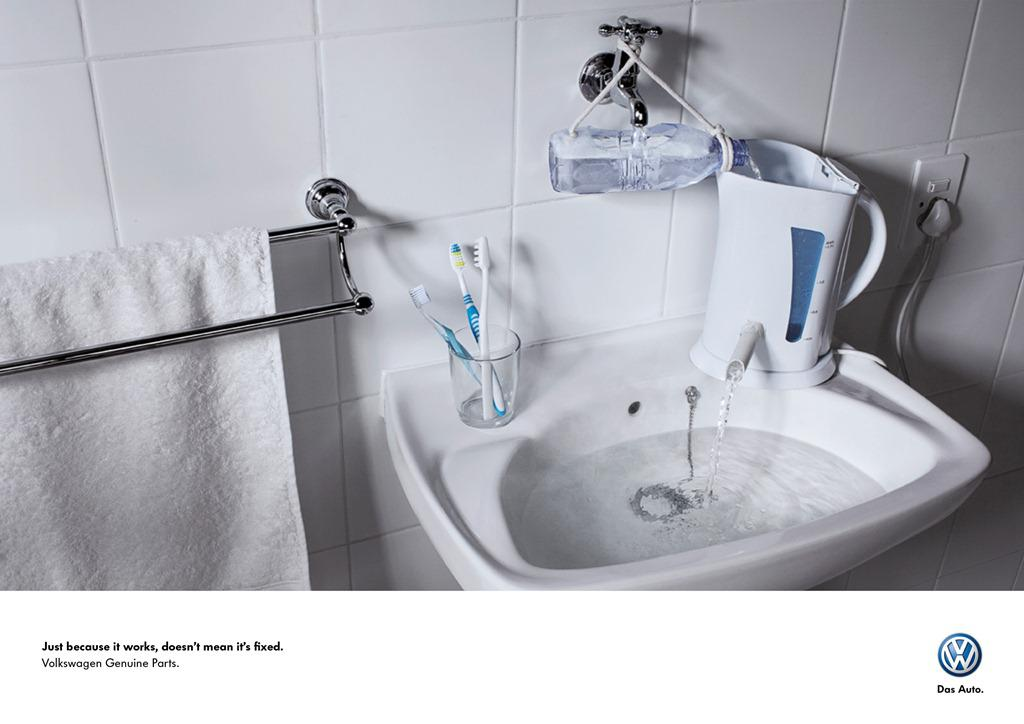
\includegraphics[width=.9\linewidth]{./images/fixed.jpg}
\end{frame}

\section{What do?}
\label{sec-7}

\begin{frame}[label=sec-7-1]{Programmers}
\begin{itemize}
\item Join the Mailing List, hang out on \emph{\#emacs} at Freenode
\item Improve your Emacs Lisp skills
\item Understand existing code, discuss and question it
\item Write demos to find better approaches to a problem
\end{itemize}
\end{frame}

\begin{frame}[label=sec-7-2]{Designers \& Writers}
“Design is about pulling things apart.” - Rich Hickey

\begin{itemize}
\item \href{https://github.com/chrisdone/structured-haskell-mode}{Gifcasts}
\item Clearer documentation
\item Suggest (UI) ideas, discuss them
\item Devise APIs and better abstractions
\end{itemize}
\end{frame}

\begin{frame}[label=sec-7-3]{Rewrite proponents}
See \href{http://www.emacswiki.org/emacs/GuileEmacs}{Guile} \href{http://git.hcoop.net/?p=bpt/emacs.git}{Emacs}
\end{frame}

\begin{frame}[label=sec-7-4]{Possible stuff to hack on}
\begin{itemize}
\item A “native” torrent client
\item Guile Emacs and things using Guile bindings (graphical browser,
video player, OpenGL, \ldots{})
\item dired
\item Window management library
\item Input methods
\item helm
\item dash.el, s.el, f.el, b.el, \ldots{}
\item my stuff
\item other people's stuff (see next slide)
\end{itemize}
\end{frame}

\begin{frame}[label=sec-7-5]{Hackers to collaborate with}
\begin{itemize}
\item \href{https://github.com/Fuco1}{Fuco1}
\item \href{https://github.com/magnars}{magnars}
\item \href{https://github.com/skeeto}{skeeto}
\item \href{https://github.com/chrisdone}{chrisdone}
\item \href{https://github.com/purcell}{purcell}
\item \href{https://github.com/thierryvolpiatto}{thierryvolpiatto}
\item \href{https://github.com/bbatsov}{bbatsov}
\item \href{https://github.com/technomancy}{technomancy}
\item \href{https://github.com/dgutov}{dgutov}
\item \ldots{}
\end{itemize}
\end{frame}

\begin{frame}[label=sec-7-6]{Conclusion}
\begin{itemize}
\item Emacs is pretty cool
\item You should totally learn to mold it to your likings
\item If you do, help out while you're at it
\item There's more than enough to be fixed
\end{itemize}
\end{frame}

\begin{frame}[label=sec-7-7]{Questions?}
“<technomancy> not making sense never stopped an intrepid elisper!”
\end{frame}
% Emacs 24.3.1 (Org mode 8.2.7c)
\end{document}